\section{Goals}

The main goal of using \textit{Linux Security Modules} in combination with WebAssembly
is to provide a finer grain customisation when choosing how to limit the permissions given
to the executable. More specifically, the desired features are:
\begin{enumerate}
  \item to give the possibility to differentiate between directories and files when giving permissions;
  \item to clearly separate different capabilities;
  \item to extend the possible set of permissions under the user's control.
\end{enumerate}

Additional desirable features include the possibility to apply exceptions to a certain rule, as well
as limiting the access to other resources in the operating systems, such as network, devices, and
inter-process communications.

Finally, usability is also taken into consideration, especially from the point of view of a user.

Note that the main purpose of these tests is not to replicate all the functionalities given by
the WebAssembly runtimes (\textit{Wasmtime} and \textit{Wasmer}), but to see how their basic features,
especially running a WebAssembly compiled binary through WASI, can be integrated and/or extended with
security tools from the Linux kernel.
This means that, for example, running a single function exported from a WebAssembly module won't be taken
into consideration.

\newpage
\section{Landlock}

For the integration with Landlock, a new project was developed, in order to provide
a custom command line interface that allowed the user to specify with more precision what
the WebAssembly binary is permitted to do on certain folders and files.

The project is open source and the code is available at \url{https://github.com/micheleberetta98/rust-wasm-landlock}.

\subsection{Code architecture and description}\label{sec:landlock-code-architecture}

The code itself is written in \textit{Rust}, and makes use of the
\textit{rust-landlock}\footnote{\url{https://github.com/landlock-lsm/rust-landlock}} crate
to communicate with Landlock and the \textit{wasmtime} and \textit{wasmtime-wasi} official
crates in order to have a runtime environment to execute a WebAssembly binary.

The project is divided into five modules, which are:
\begin{enumerate}
  \item \texttt{args}, used to define and parse the command line arguments that specify the WebAssembly binary,
        the directories to preopen, and the allowed privileges on individual folders and/or files;
  \item \texttt{landlock}, which handles the creation and update of the permissions' ruleset;
  \item \texttt{main}, the module that interfaces with the user;
  \item \texttt{path\_access}, containing a helper structure to track permission for a single path;
  \item and finally \texttt{wasm}, that communicates with the \textit{wasmtime-wasi} and the \textit{wasmtime} crates
        in order to run the provided binaries, as well as preopening directories.
\end{enumerate}

\begin{figure}[ht]
  \centering
  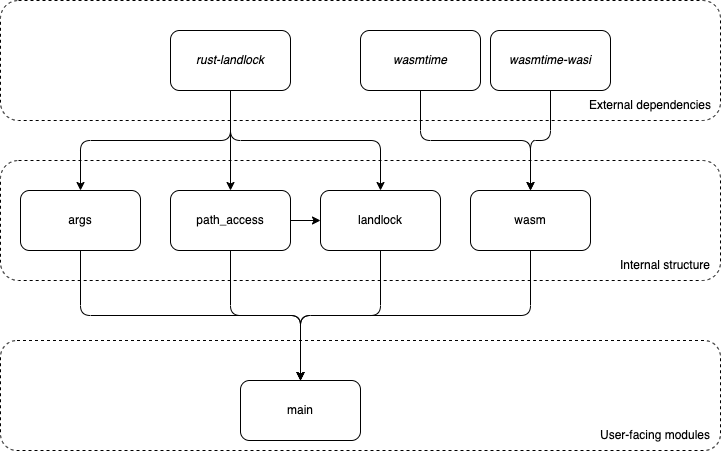
\includegraphics[width=0.9\linewidth]{rust-landlock-code-diagram.png}
  \caption{The code's architecture}
  \label{fig:rust-landlock-code-architecture}
\end{figure}

The architecture diagram is visible in Figure \ref{fig:rust-landlock-code-architecture}, where
are outlined the most important external crates and all dependencies between the modules, represented
by directed arrows.

\subsubsection{The \texttt{args} module}
\label{sec:landlock-args-module}

The main definition of this module is the \texttt{Args} struct, visible in Listing \ref{lst:arg-struct},
used to represent the command line interface that allows to specify which permissions to enable
for one or more specific paths.

\begin{code}[language=rust, caption=The \texttt{Args} struct, label=lst:arg-struct]
  #[derive(Parser, Debug)]
  #[clap(author, version, about, long_about = None)]
  pub struct Args {
    // The module to execute
    pub wasm_module: String,

    // The preopened dir(s) to pass to wasmtime
    pub dirs: Vec<String>,

    // The preopened mapped dir(s) to pass to wasmtime
    pub mapdirs: Vec<(String, String)>,

    // A list of the allowed privileges on a particular folder/file
    pub fs_allows: Vec<(String, BitFlags<AccessFs>)>,

    // Disable landlock (test only)
    pub no_landlock: bool,
  }
\end{code}

Every single field is mapped to one command line argument thanks to the \textit{clap} crates which handles the
creation and parsing of the CLI arguments structure.
Their usage and meaning is described in Table \ref{table:landlock-cli-args}.

Note that here preopening a directories does not mean it and its contents will be accessible by the
provided binary at runtime - they can still be restricted by the landlock policies. Preopening is
necessary though in order to give the possibility to access its contents.

Directories can also be \textit{mapped} - in a way similar to the one provided by the \textit{Wasmtime} command line tool,
it is possible to remap path, so that it's possible to have the binary access any arbitrary path in the system
without manually copying and/or executing it in a specific directory.

\begin{table}
  \centering
  \begin{tabular}{|l|l|l|l|}
    \hline
    \textit{Argument} & \textit{Required} & \textit{Description} \\
    \hline\hline
    \textit{WASM module} & Yes & The path to the WASM binary to run \\ \hline
    \texttt{dir} & No & All the directories to preopen \\ \hline
    \texttt{mapdir} & No & Eventual mappings between the directories \\ \hline
    \texttt{fs-allow} & No & All the permitted actions on a single path \\ \hline
    \texttt{no-landlock} & No & Used to disable the self restriction done by landlock \\
    \hline
  \end{tabular}
  \caption{All the available command line arguments}
  \label{table:landlock-cli-args}
\end{table}

The first argument is positional, and is the path where the WebAssembly module is located.

The arguments \texttt{dir}, \texttt{mapdir} and \texttt{fs-allow} can appear multiple times (or no times at all), and all the values
are then collected into a single \texttt{Vec}. In this way, it is possible to apply different restrictions on different
paths - for example, one could set some files as read-only, while another subset of files in a specific directory
could also be writable.

The \texttt{fs-allow} is made up of two parts, separated by a colon - a path to apply the restrictions to,
and a series of enabled permissions on that specific path, separated by a comma.
Each permission is mapped one-to-one to the flags provided by Landlock in a manner listed in Table \ref{table:landlock-flags}.
Moreover, there are three useful ``shortcuts'' used to represent common situations - \texttt{$\sim$read}, \texttt{$\sim$write} and \texttt{*}.

Lastly, the \texttt{no-landlock} argument is only for testing purposes - it is off by default, so that
landlock is enabled and self restriction is applied if not explicitly disabled.

\subsubsection{The \texttt{wasm} module}

This module manages a single WebAssembly binary module and forms a bridge to the \textit{wasmtime} and the \textit{wasmtime-wasi}
crates. In this project, \textit{Wasmtime} bindings are used instead of the \textit{Wasmer} ones, but both provide the
same level of functionality, albeit with a different interface.

\begin{code}[language=Rust, caption=The outline of the \texttt{wasm} module]
  pub struct WasmModule {
    bytes: Vec<u8>, ctx_builder: WasiCtxBuilder,
  }
  
  impl WasmModule {
    // Reads the WASM module and initialises the WasiCtxBuilder
    pub fn new(path: &str) -> Result<Self> {...}
  
    // Make inherit stdio to the WASM module
    pub fn use_stdio(mut self) -> Self {...}
  
    // Preopen all given directories
    pub fn preopen_all(
      mut self,
      dirs: &Vec<String>) -> Result<Self> {...}
  
    // Preopen and map all given directories
    pub fn preopen_all_map(
      mut self,
      mapdirs: &Vec<(String, String)>) -> Result<Self> {...}
  
    // Preopen (and map) a single directory
    pub fn preopen(
      mut self,
      dir: &str, guest_path: &str) -> Result<Self> {...}
  
    // Run the module
    pub fn run(self) -> Result<()> {...}
  }  
  \end{code}

Here a WASM binary is represented by a vector of bytes, and it is also handled the creation
and construction of a \textit{WASI Context}, a structure defined by the \textit{wasmtime-wasi} crate used to store
all preopened directories, eventual imports and more that will be useful to run the WebAssembly module.

Here are defined various helpers to preopen directories, both unmapped and mapped.
Most importantly, in this module it's defined how to run a WebAssembly binary - it must defined both an \textit{engine} and a \textit{linker},
as well as a \textit{store} which represents the memory of a WebAssembly module described in the previous chapter.

Note that the WebAssembly module has to have a \textit{default exported function} to run - when compiling with a WASI target,
this is usually represented by the \texttt{\_start} function, which corresponds to the \texttt{main} function in languages
such as C and Rust.

\subsubsection{The \texttt{landlock} and \texttt{path\_access} modules}

The \texttt{landlock} module is a thin wrapper around the API made available by the \textit{rust-landlock} crate.
It handles mostly ruleset creation, rule insertion, and enforces the policies before the desired WASM module is run.
The main outline of the code is visible in Listing \ref{lst:rust-landlock}.

\begin{code}[language=Rust, caption=The outline of the \texttt{landlock} module, label=lst:rust-landlock]
  pub struct Landlock {
    ruleset: RulesetCreated,
  }
  
  impl Landlock {
    // Creates a new ruleset with flags from Landlock ABI version 1
    pub fn new() -> Result<Self, RulesetError> {...}
  
    // Add a set of rules to the ruleset
    pub fn add_rules(
      mut self,
      rules: impl Iterator<Item = PathAccess>) -> Result<Self>
    {...}
  
    // Add a single rule to the ruleset
    pub fn add_rule(
      mut self,
      path_access: PathAccess) -> Result<Self>
    {...}
  
    // Self restrict the process and checks whether Landlock
    // is supported or not by the running kernel
    pub fn enforce(self) -> Result<RestrictionStatus> {...}
  }
  \end{code}

It makes use of another thin wrapper, the \texttt{PathAccess} struct defined in the \texttt{path\_access} module.
In this module, the main entity is the \texttt{PathAccess} struct, that tracks which flags as defined in Table \ref{table:landlock-flags}
are applied to a single path. The flags list starts empty, and multiple flags can be added at any times.
Moreover, this module also takes care of conversions between types required by the Landlock ABI in order
to make the code compile.

\subsection{Available permission settings}

The program allows to specify all access right flags from the first version of the Landlock
ABI\footnote{At the moment it is not possible to specify the \texttt{LANDLOCK\_ACCESS\_FS\_REFERER} in order to reparent a file hierarchy.}.

\begin{table}
  \centering
  \begin{tabular}{|l|l|}
    \hline
    \textit{Flag} & \textit{Enabled permission} \\ \hline\hline
    \texttt{X} & Execute a file \\ \hline
    \texttt{W} & Write to a file \\ \hline
    \texttt{R} & Read a file \\ \hline
    \texttt{RDir} & Open a directory or list its content \\ \hline
    \texttt{DDir} & Delete an empty directory or rename one \\ \hline
    \texttt{D} & Unlink or rename a file \\ \hline
    \texttt{MChar} & Create, rename or link a character device \\ \hline
    \texttt{MDir} & Create or rename a directory \\ \hline
    \texttt{MReg} & Create, rename or link a regular file \\ \hline
    \texttt{MSock} & Create, rename or link a socket \\ \hline
    \texttt{MFifo} & Create, rename or link a named pipe \\ \hline
    \texttt{MBlock} & Create, rename or link a block device \\ \hline
    \texttt{MSym} & Create, rename or link a symbolic link \\ \hline
    \texttt{$\sim$read} & Combination of \texttt{X}, \texttt{R} and \texttt{RDir} \\ \hline
    \texttt{$\sim$write} & Combination of all but \texttt{X}, \texttt{R} and \texttt{RDir} \\ \hline
    \texttt{*} & Enable all flags \\ \hline
  \end{tabular}
  \caption{Provided flags and corresponding Landlock permissions}
  \label{table:landlock-flags}
\end{table}

All flags are listed in Table \ref{table:landlock-flags}, and some the following examples illustrate how to combine them:
\begin{itemize}
  \item \texttt{file:R} allows only to read from \textit{file};
  \item \texttt{file:X} the combination of \texttt{.:RDir} allows the execution of \textit{file} and the listing of the current directory;
  \item \texttt{.:MReg} only allows the creation, rename or linking of regular files in the current directory;
  \item \texttt{.:R,W} and \texttt{./subdir:*} allows only reads and writes on files in the current directory, while no restrictions are
        made for \textit{subdir}.
\end{itemize}

Note that, as highlighted in Section \ref{sec:landlock-args-module}, the directories containing the files of interest
must always be preopened, even if their content is then restricted by landlock.

The Landlock self-restriction is applied after the necessary preopening of the directories,
otherwise the running process would have to always have the permissions for listing directories even if
not needed by the WASM binary.

\subsection{Advantages and disadvantages}

The main advantage that Landlock brings is simplicity. For the developer, the API is simple enough to use
to use, and it can be used in a variety of languages - the main two languages are C (used directly with the kernel libraries),
Rust as in this project, and Go\footnote{\url{https://github.com/landlock-lsm/go-landlock}}.
From the user's point of view, the provided permission flags are clear enough that it is not required to have
anything beside a basic understanding of Linux's file system permissions.
Hence, it can be used to provide a clear interface that is not so different from the one already given by
the existing runtimes.
Moreover, Landlock allows \textit{unprivileged} access control - it is not necessary to gain particular privileges
when running a binary, so the user can run a WebAssembly module in a protected environment even if they are not
in the \textit{sudoers} group.

The biggest drawback with this approach is simplicity itself. As highlighted in Section \ref{sec:intro-lsm-landlock},
there is no way to define exception - this restricts the possibilities given to the user, and makes some situations
impossible to specify. For example, if a \texttt{LANDLOCK\_ACCESS\_FS\_REMOVE\_FILE} right is given to a directory,
all files in that directory can be renamed and there is no way to prevent renaming for a specific file.
Or similarly, if a \texttt{LANDLOCK\_ACCESS\_FS\_READ\_DIR} right is given to a directory, all subdirectories
will be subjected to the same access right, so it is not possible to discriminate between subdirectories.
In addition to this, the set of capabilities is somewat limited, and mostly related to the file system.

\section{eBPF with \textit{bpfcontain}}

\subsection{Architecture}

\subsection{Available permission settings}

\subsection{Advantages and disadvantages}